\documentclass[uplatex,a4paper]{jsarticle}

\usepackage[dvipdfmx]{graphicx,xcolor}
\usepackage[T1]{fontenc}
\usepackage{otf}
\usepackage{lmodern}
\usepackage{algorithm}
\usepackage{algpseudocode}
\usepackage{siunitx}
\usepackage{float}
\usepackage{aliascnt}
\usepackage{amsmath}
\usepackage{mathtools}
\usepackage[dvipdfmx,hidelinks,hypertexnames=false]{hyperref}
\usepackage{listings}
\usepackage{subfiles}
\usepackage{caption}
\usepackage{cleveref}
\usepackage{autonum}
\usepackage{morewrites}
\usepackage[pdf,tmpdir]{graphviz}

\graphicspath{{figures/}}

\mathtoolsset{showmanualtags}

\lstset{
  basicstyle={\ttfamily},
  identifierstyle={\small},
  commentstyle={\smallitshape},
  keywordstyle={\small\bfseries},
  ndkeywordstyle={\small},
  stringstyle={\small\ttfamily},
  frame={tb},
  breaklines=true,
  columns=[l]{fullflexible},
  numbers=left,
  xrightmargin=0zw,
  xleftmargin=3zw,
  numberstyle={\scriptsize},
  stepnumber=1,
  numbersep=1zw,
  lineskip=-1ex
}

\newcounter{equationset}
\newcommand{\equationset}[1]{
  \refstepcounter{equationset}
  \noindent\makebox[\linewidth]{\theequationset: #1}
}

\renewcommand{\listfigurename}{\subsection{図一覧}}
\renewcommand{\listtablename}{\subsection{表一覧}}
\renewcommand{\listalgorithmname}{\subsection{アルゴリズム一覧}}
\renewcommand{\lstlistlistingname}{\subsection{コード一覧}}
\renewcommand{\appendixname}{}
\renewcommand{\refname}{\section{参考文献}}
\renewcommand{\figurename}{図}
\renewcommand{\tablename}{表}
\renewcommand{\theequationset}{式~\arabic{equationset}}
\renewcommand{\lstlistingname}{コード}
\makeatletter
\renewcommand{\ALG@name}{アルゴリズム}
\makeatother

\crefname{table}{表}{表}
\crefname{figure}{図}{図}
\crefname{algorithm}{アルゴリズム}{アルゴリズム}
\crefname{listing}{コード}{コード}
\crefformat{section}{#1#2節#3}
\crefformat{enumi}{#1#2.#3}

\usepackage{here}

\title{cccコンパイラのバックエンド}
\author{\href{https://keybase.io/coorde}{\texttt{coord\_e}}}
\date{2019年12月23日}

\begin{document}

\maketitle
%% \thispagestyle{empty}
%% \clearpage

% 本文
\pagenumbering{arabic}
\setcounter{page}{1}

\section{はじめに}

この記事は言語実装 Advent Calendar 2019\footnote{\url{https://qiita.com/advent-calendar/2019/lang_dev}}の23日目です。

実は、この記事の大半の文章は以前に別の目的\footnote{\url{https://twitter.com/coord_e/status/1203620846259933186?s=20}}で執筆したものです。
そういえばcccについて記事を書いていないな、ということで、少し内容を変更しつつ体裁を整えてここに公開します。
なお、ブログやスライドなどで散々「セルフホストする」「\texttt{gcc -O1}に勝つ」と豪語しておりましたが、そのどちらも達成できていません。残念。

この記事の\LaTeX ソースはGitHubに公開しています。\footnote{\url{https://github.com/coord-e/article-ccc-backend}}
また、誤字や誤謬を発見された方は\href{https://twitter.com/coord_e}{@coord\_e}までご連絡いただくかリポジトリにPull Requestを送ってくださると幸いです。

\section {概要}
\label{ccc_abstract}

\textbf{ccc}は、自分がセキュリティ・キャンプ2019\cite{seccamp19}に参加した際に開発したコンパイラだ。
C11のサブセットをコンパイルする事ができ、暗黙の型変換や初期化子、宣言子に代表される複雑な言語機能を規格に忠実に実装している。
さて、cccは効率の良いコードに効率よくコンパイルすることをテーマに開発を行った。
そのテーマのもと、出力コードの効率を高めるためにcccに実装した技術についてこの記事では説明する。
最後にベンチマークの結果を示し、実装の効果を確かめる。

\section{cccコンパイラの構成}

cccコンパイラはCのソースコードを受け取りアセンブリのコードを出力する。cccではワンパスでは行えないと思われる変形や最適化を用いているため、コンパイルの段階に応じて複数の中間表現を用いている。

一つ目の中間表現が\textbf{抽象構文木}(\textit{Abstract Syntax Tree, AST})だ。これは構文解析の結果を木構造で表現したもので、この上で意味解析が行われる。
もう一つの中間表現は\textbf{IR}と名付けた\footnote{もちろんIntermediate Representationなのだが、中間表現全体を指すわけではなく特定の段階の中間表現を指して\textbf{IR}と呼んでいる。「名付けた」と言っているのもそのためである。}。これはASTよりもアセンブリに近い構造を持っており、この上で最適化やレジスタ割り当てが行われる。IRについて\cref{ccc_ir}で詳しく説明している。

\clearpage

\begin{figure}[!ht]
  \begin{center}
    \digraph[scale=0.77]{cccarch}{
      graph [
        newrank = true;
        splines = ortho;
        nodesep = 0.3;
        ranksep = 0.3;
      ];
      node [
        style = filled;
        fillcolor = white;
        height = 0.3;
        width = 1.5;
        fixedsize = true;
        fontsize = 10;
      ];

      start [shape=ellipse, group=f, label="Input File"];

      start -> source;
      subgraph cluster_0 {
        style = "dashed, filled";
        fillcolor = lightgrey;
        color = black;
        label = "front end";
        labeljust = l;

        source  [shape=parallelogram, group=f, label="C Source"];
        tokenize  [shape=box, group=f, label="Tokenize"];
        tokens  [shape=parallelogram, group=f, label="Tokens"];
        parse  [shape=box, group=f, label="Parse"];
        ast1  [shape=parallelogram, group=f, label="AST"];
        sema  [shape=box, group=f, label="Semantic Analysis"];
        ast2  [shape=parallelogram, group=f, label="AST"];

        source -> tokenize -> tokens -> parse -> ast1 -> sema -> ast2  [weight=10];
      }
      ast2 -> irgen [weight=0];

      subgraph cluster_1 {
        style = "dashed, filled";
        fillcolor = lightgrey;
        color = black;
        label = "back end";
        labeljust = l;

        irgen [shape=box, group=b1, label="IR Generation"];
        ir1 [shape=parallelogram, group=b1, label="IR"];
        mem2reg [shape=box, group=b1, label="Mem2Reg"];
        ir2 [shape=parallelogram, group=b1, label="IR"];
        arch [shape=box, group=b1, label="Target Conversion"];
        ir3 [shape=parallelogram, group=b1, label="IR"];
        liveness [shape=box, group=b2, label="Liveness Analysis"];
        ir4 [shape=parallelogram, group=b2, label="IR"];
        regalloc [shape=box, group=b2, label="Register Allocation"];
        ir5 [shape=parallelogram, group=b2, label="IR"];
        codegen [shape=box, group=b2, label="Code Generation"];
        asm [shape=parallelogram, group=b2, label="x64 Assembly"];

        irgen -> ir1 -> mem2reg -> ir2 -> arch -> ir3  [weight=10];
        ir3 -> liveness [weight=0];
        liveness -> ir4 -> regalloc -> ir5 -> codegen -> asm [weight=10];

      }
      asm -> end;

      end [shape=oval, group=b2, label="Output"];

      { rank=same; tokenize -> irgen -> liveness [style=invis]; }
    }
    \caption{cccコンパイラ全体の構成}
    \label{ccc_arch}
  \end{center}
\end{figure}

\cref{ccc_arch}はコンパイラ全体の構成を表している。cccコンパイラの内部パスはソースコードからASTを扱う\textbf{フロントエンド}(\textit{front end})と、IRを扱う\textbf{バックエンド}(\textit{back end})に概念上分類することができる。
フロントエンドではソースコードに対して字句解析と構文解析を行ってASTを生成し、ASTの上で意味解析を行ったのちIRを生成する。バックエンドは生成されたIRの上でコード変形や最適化を行い、最終的に一般的なアセンブラで処理可能な形式のx86\_64アセンブリを生成する。

なお、バックエンドは今日ではLLVM\cite{TheLLVM}に代表されるようなコンパイラ基盤で置き換える事ができる。
しかしcccでは低レイヤ・オタク特有のいわゆる``一から作りたい欲求''に身を任せ、バックエンドを既存のフレームワークを使用せずに自作している。
この記事では主にcccコンパイラのバックエンドに焦点を絞って説明する。

この記事では構文解析に代表されるようなフロントエンドについては説明しない。理論的な側面については\cite{av2009コンパイラ}が詳しい。また、フロントエンドに限らないが、実装から入る場合は\cite{ruicompilerbook}が非常に良いオンラインブックであるとして有名である。

\clearpage
\section{IR}
\label{ccc_ir}

IRは出力先のネイティブコードに近い構造を持つように設計した。IR内では関数が単位となっており\footnote{翻訳単位に対応するIRは、翻訳単位内で定義された複数の関数IRが集まったものである}、これを\textbf{関数IR}と呼ぶことにする。IRに対する操作も基本的に関数IR単位で行われる。
関数IRはメタデータを除けばIR命令の列である。IR命令列は\textbf{基本ブロック}(\textit{basic block})に分割されており、各基本ブロックは\textbf{後続節}(\textit{predecessors})と\textbf{先行節}(\textit{successors})の情報を保持している。
これらの情報から基本ブロックは\textbf{制御フローグラフ}(\textit{Control Flow Graph, CFG})を構成する(\cref{ccc_cfg_fig})。

IR命令はレジスタをオペランドにとる。cccのIR上のレジスタには以下の3つの種類がある。
\begin{itemize}
  \item \textbf{仮想レジスタ}(\textit{virtual register})は、IR生成の際に使われる、無限個存在するレジスタ。
  \item \textbf{物理レジスタ}(\textit{physical register})は、レジスタ割り当てが終わったレジスタ。有限個であり、出力コードのレジスタに一対一で対応している。
  \item \textbf{固定レジスタ}(\textit{fixed regitser})は、\cref{archconv}の変換で生成される、割り当てられる物理レジスタが事前に決まっている仮想レジスタ。
\end{itemize}

IRを表す図中では、n番目の仮想レジスタを\texttt{v}$n$、n番目の物理レジスタを\texttt{r}$n$、\texttt{r}$n$に割り当てられる$m$番目の固定レジスタは\texttt{f(v$m$:r$n$)}と表記する。

さて、IR命令の命令セットを\cref{tb:ccc_isa}に示す。
なお、今後の表やアルゴリズムでは命令の出力オペランドを$rd$、n番目の入力オペランドを$ra[n]$と表記する。

表には記載がないが、これらの他に\texttt{BIN\_IMM}といった片方のオペランドに定数をとる命令や\texttt{BR\_CMP}といった複合命令が実装されている。これらは主にレジスタ上のデータの流れを用いた最適化である\textbf{データフロー最適化}で効率的なアセンブリを出力するために用いている。

IRはASTから生成され、IRの上で最適化やレジスタ割り当てが行われたのちにコード生成パスでx86\_64のアセンブリに変換される。

\begin{figure}[hb]
  \begin{minipage}{0.50\hsize}
    \centering
    \begin{verbatim}
int main() {
  int i = 0;
  for (int j = 0; j < 10; j++) {
    if (j < 3)
      continue;
    i = i + 1;
  }
  return i;
}
    \end{verbatim}
    \caption*{元のソースコード}
  \end{minipage}
  \begin{minipage}{0.50\hsize}
    \centering
    \input{figures/cfg.gv}
    \caption*{対応するIR}
  \end{minipage}
  \caption{cccが出力するIR(CFG)の例}
  \label{ccc_cfg_fig}
\end{figure}

\begin{table}[hp]
  \centering
  \begin{tabular}{llll}
    \multicolumn{2}{l}{命令} & 説明 & 効果 \\ \hline\hline
    \texttt{rd =}&\texttt{MOV ra[0]} & レジスタの代入 & $rd \gets ra[0]$ \\
    \texttt{rd =}&\texttt{IMM $imm$} & 即値$imm$の代入 & $rd \gets imm$ \\
    \texttt{rd =}&\texttt{BIN $op$ ra[0] ra[1]} & 二項演算 & $rd \gets ra[0] \mathbin{op} ra[1]$ \\
    \texttt{rd =}&\texttt{UNA $op$ ra[0]} & 単項演算 & $rd \gets \mathrel{op} ra[0]$ \\
    \texttt{rd =}&\texttt{ARG $idx$} & $idx$番目の引数の代入 & $rd \gets $ value of $idx$-th argument \\
    &\texttt{RET ra[0]} & 関数から値を返す & return $ra[0]$ \\
    &\texttt{RET} & 関数から返る & return $void$ \\
    \texttt{rd =}&\texttt{SEXT ra[0]} & 整数の符号拡張 & $rd \gets$ extend $ra[0]$ to the size of $rd$ \\
    \texttt{rd =}&\texttt{TRUNC ra[0]} & 整数の切り詰め & $rd \gets$ trunc $ra[0]$ to the size of $rd$ \\
    &\texttt{STORE ra[0] ra[1]} & アドレスに値を格納 & $*ra[0] \gets ra[1]$ \\
    \texttt{rd =}&\texttt{LOAD ra[0]} & アドレスから値をロード & $rd \gets *ra[0]$ \\
    &\texttt{LABEL $label$} & ラベル & a label named $label$ \\
    &\texttt{BR ra[0] $then$ $else$} & 値に応じてラベルにジャンプ & if $ra[0]$ jump to $then$ else to $else$ \\
    &\texttt{JUMP $label$} & 指定されたラベルにジャンプ & unconditionally jump to $label$ \\
    \texttt{rd =}&\texttt{CALL ra[0] ra[1] ra[n]...} & 関数呼び出し & $rd \gets$ call $ra[0]$ with $ra[n]...$ \\
    \texttt{rd =}&\texttt{STACK\_ADDR $stack\_idx$} & スタック上の位置のアドレス取得 & $rd \gets $ an address of $stack\_idx$ \\
    \texttt{rd =}&\texttt{GLOABL\_ADDR $kind$ $name$} & グローバルな名前のアドレス取得 & $rd \gets $ an address of $name$ \\
    &\texttt{STACK\_STORE $stack\_idx$ ra[0]} & スタックに値を格納 & $*stack\_idx \gets ra[0]$ \\
    \texttt{rd =}&\texttt{STACK\_LOAD $stack\_idx$} & スタックから値をロード & $rd \gets *stack\_idx$
  \end{tabular}
  \caption{cccのIR命令セット(一部)}
  \label{tb:ccc_isa}
\end{table}

\clearpage
\section{ターゲット固有IRへの変換}
\label{archconv}

ここでは\cref{ccc_arch}で「Target Conversion」と表記されている変換について説明する。

アーキテクチャやABI(ここでは二つをまとめてターゲットと呼ぶ)によっては、命令がある決まったレジスタを使用することがある。
例えばx86\_64アーキテクチャ\cite{guide2011intel}において除算命令\texttt{div}は被除数を\texttt{rax}にとり、商を\texttt{rax}に格納する。
またSystem V ABI\cite{SystemV}において\texttt{call}命令は\texttt{rdi, rsi, rdx, rcx, r8, r9}に引数をとり戻り値を\texttt{rax}を格納する。
こういった特別に扱われるレジスタをここでは\textbf{特殊レジスタ}と呼ぶ。
また、x86\_64では\texttt{add, sub}などのいくつかの命令において演算の左辺と演算結果が同じレジスタでなければならないという制約がある。

一方で、cccのIRでは\cref{tb:ccc_isa}からわかる通りオペランドのレジスタに特に制限を設けていない。
そのため、単純な実装ではコード生成時に適切に\texttt{mov}命令を挿入して決まったレジスタを使うようにすることになる。
しかし、この方法では特殊レジスタを汎用的に使うことができず、レジスタ割り当てに使えるレジスタの数が制限されてしまう。
また、一つのIR命令に対応するアセンブリ命令が多くなってしまうと最適化の効果が制限されてしまうことも予想された。

そこで、cccではレジスタ割り当て前にIR上でターゲット特有の変換を行うことでこれらの問題を解決している。
これはIR上で固定レジスタへの\texttt{MOV}命令を生成することでコード生成時に正しいレジスタが使用されていることを保証しながらIR上で特殊レジスタの使用を表現するものだ。
こうすることでレジスタ割り当ての時点で特殊レジスタの使用が把握できるため、特殊レジスタが使われていない部分では通常のレジスタとして割り当てに使用できるようになる。
\cref{ccc_arch_fig}にこの変換の例を示す。関数呼び出しや除算が固定レジスタを使うように変換されているのが見て取れる。

\begin{figure}[h]
  \begin{minipage}{0.50\hsize}
    \centering
    \input{figures/before_arch.gv}
    \caption*{変換前}
  \end{minipage}
  \begin{minipage}{0.50\hsize}
    \centering
    \input{figures/after_arch.gv}
    \caption*{変換後}
  \end{minipage}
  \caption{ターゲット固有IRへの変換前後のIRの変化例}
  \label{ccc_arch_fig}
\end{figure}

\clearpage
\section{最適化}
\label{optimization}

効率の良いコードを出力するため、最適化を行った。

cccではデッドコード削除やコピー伝播に代表されるデータフロー最適化やAST上の定数畳み込みなどを実装しているが、ここではそれらについては説明しない。
特にデータフロー最適化について、技術書展8に(もし当選すれば)OtakuAssembly\footnote{\url{https://twitter.com/OtakuAssembly}}で(もし書き切る事ができたら)記事を出すので、ぜひそちらを楽しみにしていてください。

さて、ここでは\texttt{LOAD}/\texttt{STORE}以外の操作を受けていないスタック上の領域をレジスタで置き換える最適化について説明する。
このパスを\textbf{mem2reg}と名付けた。\footnote{LLVMに同じような名前の最適化パスがあり、実際それから名前は着想を得たが、最適化の内容については関連はないものとする}
mem2regで使用および実装したアルゴリズムを\cref{algmem2reg}に示す。

\begin{algorithm}[h]
\caption{Naive mem2reg}\label{algmem2reg}
\begin{algorithmic}[1]
\Procedure{Mem2Reg}{IR instructions $insts$}
  \State $targets \gets \Call{CollectUses}{insts}$
  \State \Call{ReplaceInstructions}{$insts, targets$}
\EndProcedure
\end{algorithmic}
\end{algorithm}

ここではアドレスとして用いられているレジスタを\textbf{アドレスレジスタ}(\textit{address register})と呼ぶ。
\texttt{LOAD}/\texttt{STORE}命令のアドレスの位置にあるオペランドとして使われているレジスタがアドレスレジスタである。

\textsc{CollectUses}(\cref{algmem2regcollect})でアドレスレジスタのうち、置き換え可能なものを求める。
ここではアドレスレジスタを\texttt{candidates}に集めながら、\texttt{LOAD}/\texttt{STORE}以外の操作を受けているレジスタを\texttt{excluded}に集めている。
また、\texttt{STACK\_ADDR}命令で代入されているレジスタを個別に\texttt{in\_stack}に集めている。

さて、置き換え可能なアドレスレジスタは、以下の3条件を満たしているものである。
\begin{enumerate}
  \item \label{mem2regenum:1}スタックのアドレスを保持している
  \item \label{mem2regenum:2}\texttt{LOAD}/\texttt{STORE}以外の操作を受けていない
  \item \label{mem2regenum:3}置き換え不可能なアドレスレジスタと同じスタック位置を共有していない
\end{enumerate}
\cref{mem2regenum:1}, \cref{mem2regenum:2}を満たすアドレスレジスタの集合は、$(\texttt{candidates} - \texttt{excluded}) \cap {\texttt{in\_stack}}$で求められる。\footnote{集合の実装にBit Vectorと呼ばれるデータ構造を使用しており、集合の演算が非常に効率的に行える}
そして\cref{mem2regenum:3}を満たさないものを除外するために、置き換え不可能なアドレスレジスタのスタック位置の集合を求め、そのあとにそれを共有しているものを除外するというナイーブな方法をとった。

そして、置き換え可能なアドレスレジスタが求められたのち、\textsc{ReplaceInstructions}(\cref{algmem2regreplace})で命令をレジスタを使うように書き換えている。

\begin{algorithm}
\caption{Collecting uses of address registers}\label{algmem2regcollect}
\begin{algorithmic}[1]
\Function{CollectUses}{list of IR instructions $insts$}
  \State $candidates, excluded, in\_stack \gets \emptyset$
  \ForAll{instruction $inst$ in $insts$}
    \If{$inst$ is \texttt{STACK\_ADDR}}
      \State $in\_stack \gets in\_stack \cup{ \{inst.rd\} }$
      \State $assoc\_areas[inst.rd] \gets inst.stack\_idx$
    \ElsIf{$inst$ is \texttt{LOAD}}
      \State $candidates \gets candidates \cup{ \{inst.ra[0]\} }$
      \State $excluded \gets excluded \cup{ \{inst.rd\} }$
    \ElsIf{$inst$ is \texttt{STORE}}
      \State $candidates \gets candidates \cup{ \{inst.ra[0]\} }$
      \State $excluded \gets excluded \cup{ \{inst.ra[1]\} }$
    \Else
      \ForAll{register $r$ in $inst.ra$}
        \State $excluded \gets excluded \cup{ \{r\} }$
      \EndFor
      \If{$inst$ has $inst.rd$}
        \State $excluded \gets excluded \cup{ \{inst.rd\} }$
      \EndIf
    \EndIf
  \EndFor
  \State \textbf{return} \Call{ComputeReplaceable}{$candidates, excluded, in\_stack$}
\EndFunction
\Function{ComputeReplaceable}{set of registers $candidates$, $excluded$, $in\_stack$}
  \State $replaceable \gets (candidates - excluded) \cap {in\_stack}$
  \State $ex\_areas \gets \emptyset$
  \ForAll {register $r$ in $\overline{replaceable}$}
    \If{$r$ found in $assoc\_areas$}
      \State $s \gets assoc\_areas[r]$
      \State $ex\_areas \gets ex\_areas \cup{\{s\}}$
    \EndIf
  \EndFor
  \ForAll {register $r$ in $replaceable$}
    \State $s \gets assoc\_areas[r]$
    \If{$s\in{ex\_areas}$}
      \State $replaceable \gets replaceable - \{r\}$
    \Else
      \If{$s$ not found in $replaced\_regs$}
        \State $replaced\_regs[s] \gets$ new replacement register
      \EndIf
    \EndIf
  \EndFor
\EndFunction
\end{algorithmic}
\end{algorithm}

\begin{algorithm}
\caption{Replace instructions}\label{algmem2regreplace}
\begin{algorithmic}[1]
\Procedure{ReplaceInstructions}{list of IR instructions $insts$, set of registers $targets$}
  \ForAll{instruction $inst$ in $insts$}
    \If{$inst$ is \texttt{STACK\_ADDR}}
      \If{$inst.rd\in{targets}$}
        \State remove $inst$ from $insts$
      \EndIf
    \ElsIf{$inst$ is \texttt{LOAD}}
      \If{$inst.ra[0]\in{targets}$}
        \State $s \gets assoc\_areas[inst.ra[0]]$
        \State $r \gets replaced\_regs[s]$
        \State replace $inst$ with \texttt{'$inst.rd$ = MOVE $r$'} in $insts$
      \EndIf
    \ElsIf{$inst$ is \texttt{STORE}}
      \If{$inst.ra[0]\in{targets}$}
        \State $s \gets assoc\_areas[inst.ra[0]]$
        \State $r \gets replaced\_regs[s]$
        \State replace $inst$ with \texttt{'$r$ = MOVE $inst.ra[1]$'} in $insts$
      \EndIf
    \EndIf
  \EndFor
\EndProcedure
\end{algorithmic}
\end{algorithm}

\cref{ccc_mem2reg_fig}にこの最適化による変形の例を示す。一部のスタックに対する操作がレジスタに置き換わっていることが見て取れる。
この最適化による出力コードの効率の変化については\cref{ccc_performance}で検討する。

\begin{figure}[h]
  \begin{minipage}{0.50\hsize}
    \centering
    \input{figures/before_mem2reg.gv}
    \caption*{最適化前}
  \end{minipage}
  \begin{minipage}{0.50\hsize}
    \centering
    \input{figures/after_mem2reg.gv}
    \caption*{最適化後}
  \end{minipage}
  \caption{mem2reg最適化前後のIRの変化例}
  \label{ccc_mem2reg_fig}
\end{figure}

\clearpage
\section{レジスタ割り当て}
\label{ccc_regalloc}

今回、高速なコードを出力させるため、出力コードはレジスタマシンとして出力することにした。
そのために、レジスタ割り当てを行う。一般的なプロセッサにおいてレジスタは有限だ。例えばx86\_64においては16本、そのうち汎用的に使えるのは14本しかない。
すなわち、全ての値をレジスタに保存しておくことはできない。値を保存するレジスタが足りなくなった時に、レジスタの代わりにスタックの領域を使う。これを\textbf{spill}と呼ぶ。
spillされたレジスタは使用時にスタックから読み込まれ、値の変更時にスタックに書き戻される。
レジスタへのアクセスはメモリへのアクセスと比べて非常に高速であるため、頻繁にアクセスされる値をレジスタに、そうでない値をメモリに配置することが出力コードの効率向上に繋がる。

一方で最適なレジスタの割り当てを求める問題はNP完全であることが知られている。そこで、コンパイル時間と実行時の効率のバランスが取れたアルゴリズムが考案されてきた。
そのよく知られた例の一つが、レジスタ割り当てをグラフ彩色問題とみなす方法\cite{chaitin1981register}である。しかしこの方法はコンパイル時間が長くかかり、また実装が複雑になるなどの点で今回は採用しなかった。

cccでは、Linear scan register allocationを実装した。これはPolettoらによって\cite{poletto1997tcc}で使われたレジスタ割り当てアルゴリズムだ。
これはグラフ彩色による手法に比べて割り当てにかかる計算量が少なくて済む上に、同じぐらい効率の良いコードを出力できる。

cccの実装では、まずIR上でbackward data-flow analysis\cite{av2009コンパイラ}を行い、仮想レジスタの生存区間を求めたのち、レジスタ割り当てを行う。
生存区間解析の実装はほぼ\cite{wimmer2004linear}で使われているアルゴリズムの通りである。
レジスタ割り当てのアルゴリズムは\cite{poletto1999linear}を元にしたが、固定レジスタを扱うために一部変更を加えている。
実際に使用したアルゴリズムを\cref{algalloc}に示す。

\begin{algorithm}[h]
\caption{Register allocation}\label{algalloc}
\begin{algorithmic}[1]
\Procedure{RegAlloc}{list of IR instructions $insts$, list of intervals $ivs$}
   \State sort $ivs$ by increasing start point
   \State \Call{WalkIntervals}{$ivs$}
   \State assign results in $result$ to every register in $insts$
\EndProcedure
\end{algorithmic}
\end{algorithm}

このアルゴリズムでは、割り当てに際して三つのグローバルな変数を持っている。

\begin{itemize}
  \item \texttt{available}は現在利用可能な物理レジスタのリスト\footnote{\texttt{available}と\texttt{active}には先頭と末尾へのポインタを保持した双方向リンクリストを用い、要素の挿入/取得が定数時間で行えるようにしている}で、後に述べる優先度でソートされている。
  \item \texttt{active}は現在使われている仮想レジスタのリストで、生存区間の終了が遅い順にソートされている。
  \item \texttt{result}は仮想レジスタから割り当てられた物理レジスタへの写像\footnote{物理レジスタと仮想レジスタには自然数のインデックスがついているので、レジスタからの写像は配列で実装されている}。
\end{itemize}

これらの変数に対する操作は、\textsc{AllocSpecificReg}(\cref{algallocreg})と\textsc{ReleaseReg}(\cref{algreleasereg})の二つの操作に抽象化されている。
アルゴリズム本体ではこれら二つの操作とspillを適切な条件で行うことで、割り当てを行なっている。
また、\texttt{available}は次の条件もとソートされている。(\cref{algcomprio})
なお、関数呼び出しで保存されないレジスタ\footnote{System V ABIではrax, rdi, r9など}のことを\textbf{scratch register}と呼ぶ。

\begin{enumerate}
  \item 現在の関数内の固定レジスタで使用されている物理レジスタより、そうでない物理レジスタを優先する。
  \item 現在の関数が関数呼び出しを含むならば、scratch registerでない物理レジスタを優先する。そうでないならばscratch registerを優先する。
\end{enumerate}

\textsc{AllocSpecificReg}(\cref{algallocreg})からわかる通り、割り当てる物理レジスタは\texttt{available}の先頭から選ばれる。これにより、\cref{algcomprio}で優先されているものから順に割り当てられる物理レジスタが選出されることになる。

\begin{algorithm}
\caption{Allocation priority}\label{algcomprio}
\begin{algorithmic}[1]
  \Ensure return $true$ if $r1$ is preferred than $r2$
\Function{ComparePriority}{physical register $r1$, physical register $r2$}
  \If{$r1$ is used in fixed registers in this function}
    \State \textbf{return} $false$
  \EndIf
  \If{$r2$ is used in fixed registers in this function}
    \State \textbf{return} $true$
  \EndIf
  \If{there are some call instruction in this function}
    \State \textbf{return} $\mathord{!}is\_scratch[r1] \mathbin{\&} is\_scratch[r2]$
  \Else
    \State \textbf{return} $is\_scratch[r1] \mathbin{\&} \mathord{!}is\_scratch[r2]$
  \EndIf
\EndFunction
\end{algorithmic}
\end{algorithm}

さて、Linear scan register allocationは、生存区間に対する一回の走査によって行われる。
\cref{algwalkintv}に走査部分のアルゴリズムを示す。また、spill関連のアルゴリズムを\cref{algspill}に示す。
固定レジスタの割り当てでは、必要な物理レジスタがすでに割り当てられていた場合にそれをspillすることで物理レジスタを確保する。また、spillの対象のレジスタを選ぶ際に固定レジスタを避けるようにしている。それ以外はほぼ\cite{poletto1999linear}の通りである。

\cref{ccc_alloc_fig}にレジスタ割り当ての例を示す。全て仮想レジスタが物理レジスタに割り当てられているだけでなく、変換前に固定レジスタだったレジスタは、正しく指定されたレジスタに割り当てられていることが見て取れる。

\begin{figure}[h]
  \begin{minipage}{0.50\hsize}
    \centering
    \input{figures/before_regalloc.gv}
    \caption*{割り当て前}
  \end{minipage}
  \begin{minipage}{0.50\hsize}
    \centering
    \input{figures/after_regalloc.gv}
    \caption*{割り当て後}
  \end{minipage}
  \caption{レジスタ割り当て前後のIRの変化例}
  \label{ccc_alloc_fig}
\end{figure}

\begin{algorithm}
\caption{Walking intervals}\label{algwalkintv}
\begin{algorithmic}[1]
\Procedure{WalkIntervals}{list of intervals $ivs$}
   \State $active \gets \{\}$
   \ForAll{usable physical register $phy$}
     \State add $phy$ to $available$ \Comment{sorted by \Call{ComparePriority}{}}
   \EndFor
   \ForAll{interval $iv$ in $ivs$}
     \State \Call{ExpireOldIntervals}{$iv$}
     \If{$iv.reg$ is a virtual register}
       \If{$available = \{\}$}
         \State \Call{SpillAtInterval}{$iv$}
       \Else
         \State \Call{AllocFreeReg}{$iv.reg$}
       \EndIf
     \ElsIf{$iv.reg$ is a fixed register}
       \If{any virtual register is allocated to $iv.reg.phy\_reg$}
         \State $v \gets$ virtual register allocated to $iv.reg.phy\_reg$
         \State \Call{SpillReg}{$v$}
       \EndIf
       \State \Call{AllocSpecificReg}{$iv.reg, iv.reg.phy\_reg$}
     \EndIf
   \EndFor
\EndProcedure
\Procedure{ExpireOldIntervals}{interval $iv$}
  \ForAll{virtual register $r$ in $active$} \Comment{in order of increasing end point}
    \State $intv \gets$ interval of $r$
    \If {$intv.to \ge iv.to$}
      \State \textbf{return}
    \EndIf
    \State \Call{ReleaseReg}{$r$}
  \EndFor
\EndProcedure
\Procedure{AllocFreeReg}{virtual register $reg$}
  \State $phy \gets$ first register in $available$ \Comment{the most prioritized register is selected here}
  \State \Call{AllocSpecificReg}{$reg, phy$}
\EndProcedure
\end{algorithmic}
\end{algorithm}

\begin{algorithm}
\caption{Spilling}\label{algspill}
\begin{algorithmic}[1]
\Procedure{SpillAtInterval}{interval $iv$}
  \State $spill \gets$ last non-fixed register in $active$ \Comment{active register with latest end point is selected here}
  \State $spill\_intv \gets$ interval of $spill$
  \If{$spill\_intv.to > iv.to$}
    \State $r \gets result[spill]$\Comment{physical register allocated to $phy$}
    \State \Call{SpillReg}{$spill$}
    \State \Call{AllocSpecificReg}{$spill, r$}
  \Else
    \State \Call{SpillReg}{$reg$}
  \EndIf
\EndProcedure
\Procedure{SpillReg}{virtual register $reg$}
  \If{$reg$ found in $result$}\Comment{if $reg$ is allocated to a physical register}
    \State \Call{ReleaseReg}{$reg$}
  \EndIf
  \State allocate new stack location to $reg$
\EndProcedure
\end{algorithmic}
\end{algorithm}

\begin{algorithm}
\caption{Allocation of specific register}\label{algallocreg}
\begin{algorithmic}[1]
  \Require no virtual register is allocated to $phy$
  \Ensure $reg$ is allocated to $phy$
\Procedure{AllocSpecificReg}{virtual register $reg$, physical register $phy$}
  \State $result[reg] \gets phy$
  \State remove $phy$ from $available$
  \State add $reg$ to $active$ \Comment{sorted by increasing end point}
\EndProcedure
\end{algorithmic}
\end{algorithm}

\begin{algorithm}
\caption{Release of virtual register}\label{algreleasereg}
\begin{algorithmic}[1]
  \Require $reg$ is allocated to a physical register
  \Ensure $reg$ is released
\Procedure{ReleaseReg}{virtual register $reg$}
  \State $phy \gets result[reg]$
  \State remove $reg$ from $active$
  \State add $phy$ to $available$ \Comment{sorted by \Call{ComparePriority}{}}
  \EndProcedure
\end{algorithmic}
\end{algorithm}

\clearpage
\section{評価}
\label{ccc_performance}

\cref{archconv}の変換や\cref{optimization}の最適化の効果を確かめるために、ベンチマークを行った。

ベンチマーク環境は以下の通り。
\begin{itemize}
  \item CPU: AMD Ryzen 7 2700
  \item RAM: 32GB
  \item kernel: 5.2.8-arch1-1-ARCH
  \item OS: Arch Linux
  \item gcc: 9.1.0
\end{itemize}

今回は三種類のプログラムをベンチマークに用いた。それぞれ次の通り。
\begin{itemize}
  \item 14queen - N-queen問題のn=14の場合の全ての解を求める
  \item sort - 30000000個のランダムな要素からなる配列のマージソート
  \item pi - 円周率を200000桁求める
\end{itemize}

以下の5種のコンパイラにこれらのプログラムをコンパイルさせ、コンパイル時間と実行時間、および出力コードの行数を計測した。
計測はそれぞれ8回行い、平均値を算出した。

\begin{enumerate}
   \item 固定レジスタを導入する前のccc (naive)
   \item \label{enum:cccbetteralloc} 固定レジスタを導入し14本のレジスタを活用できるようになったccc (better\_alloc)
   \item \cref{enum:cccbetteralloc}にmem2reg最適化を導入したccc (mem2reg)
   \item gcc -O0
   \item gcc -O1
\end{enumerate}

\clearpage
\paragraph{コンパイル時間}

コンパイル時間のベンチマーク結果を\cref{ccc_bench_compile}と\cref{ccc_bench_compile_graph}に示す。

\begin{table}[h]
  \centering
  \begin{tabular}{l|rl|rl|rl|rl|rl}
    &\multicolumn{10}{c}{実行時間, 秒 (gcc -O0との比)} \\ \hline
    &\multicolumn{2}{c|}{naive}&\multicolumn{2}{c|}{better\_alloc}&\multicolumn{2}{c|}{mem2reg}&\multicolumn{2}{c|}{gcc -O0}&\multicolumn{2}{c}{gcc -O1} \\ \hline\hline
    14queen&0.010&(0.35)&0.009&(0.29)&0.010&(0.35)&0.029&(1.00)&0.044&(1.50) \\
    sort&0.012&(0.48)&0.011&(0.44)&0.011&(0.47)&0.024&(1.00)&0.047&(1.91) \\
    pi&0.007&(0.24)&0.006&(0.19)&0.010&(0.34)&0.030&(1.00)&0.031&(1.03) \\
  \end{tabular}
  \caption{ベンチマーク結果: コンパイル時間}
  \label{ccc_bench_compile}
\end{table}

\begin{figure}[h]
  \centering
  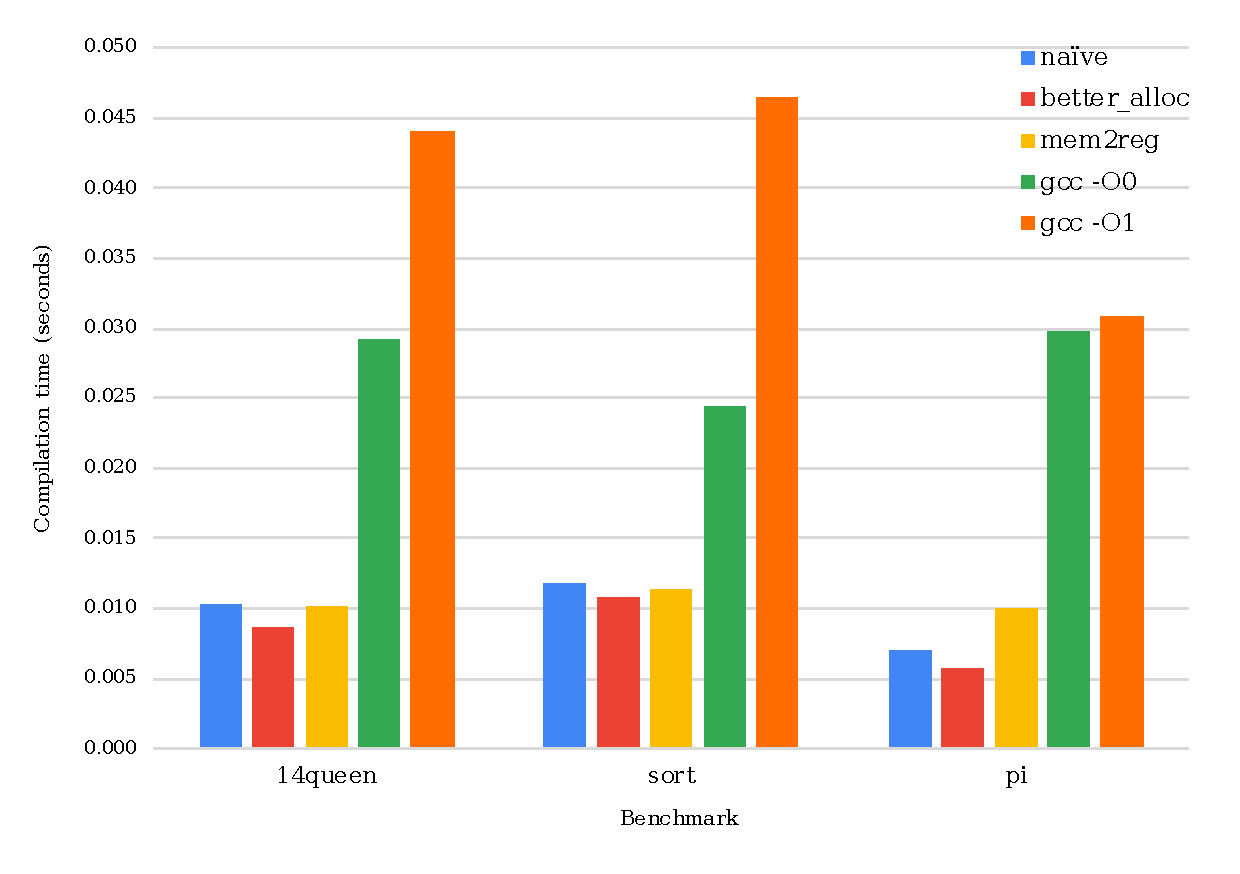
\includegraphics[width=15cm]{graph2.pdf}
  \caption{コンパイラごとのコンパイル時間の比較}
  \label{ccc_bench_compile_graph}
\end{figure}

\clearpage
\paragraph{実行時間}

実行時間のベンチマーク結果を\cref{ccc_bench_run}と\cref{ccc_bench_run_graph}に示す。なお、naiveのsortについてはその時点でのcccの実装にバグがあり実行時エラーが生じているため正常な計測ができていない。

\begin{table}[h]
  \centering
  \begin{tabular}{l|rl|rl|rl|rl|rl}
    &\multicolumn{10}{c}{実行時間, 秒 (gcc -O0との比)} \\ \hline
    &\multicolumn{2}{c|}{naive}&\multicolumn{2}{c|}{better\_alloc}&\multicolumn{2}{c|}{mem2reg}&\multicolumn{2}{c|}{gcc -O0}&\multicolumn{2}{c}{gcc -O1} \\ \hline\hline
    14queen&24.4&(2.27)&25.9&(2.41)&22.7&(2.11)&10.8&(1.00)&5.59&(0.52) \\
    sort&0.30&(0.04)&12.2&(1.55)&11.2&(1.43)&7.86&(1.00)&3.65&(0.46) \\
    pi&23.8&(1.26)&18.9&(1.00)&14.3&(0.76)&18.9&(1.00)&0.00&(0.00) \\
  \end{tabular}
  \caption{ベンチマーク結果: 実行時間}
  \label{ccc_bench_run}
\end{table}

\begin{figure}[h]
  \centering
  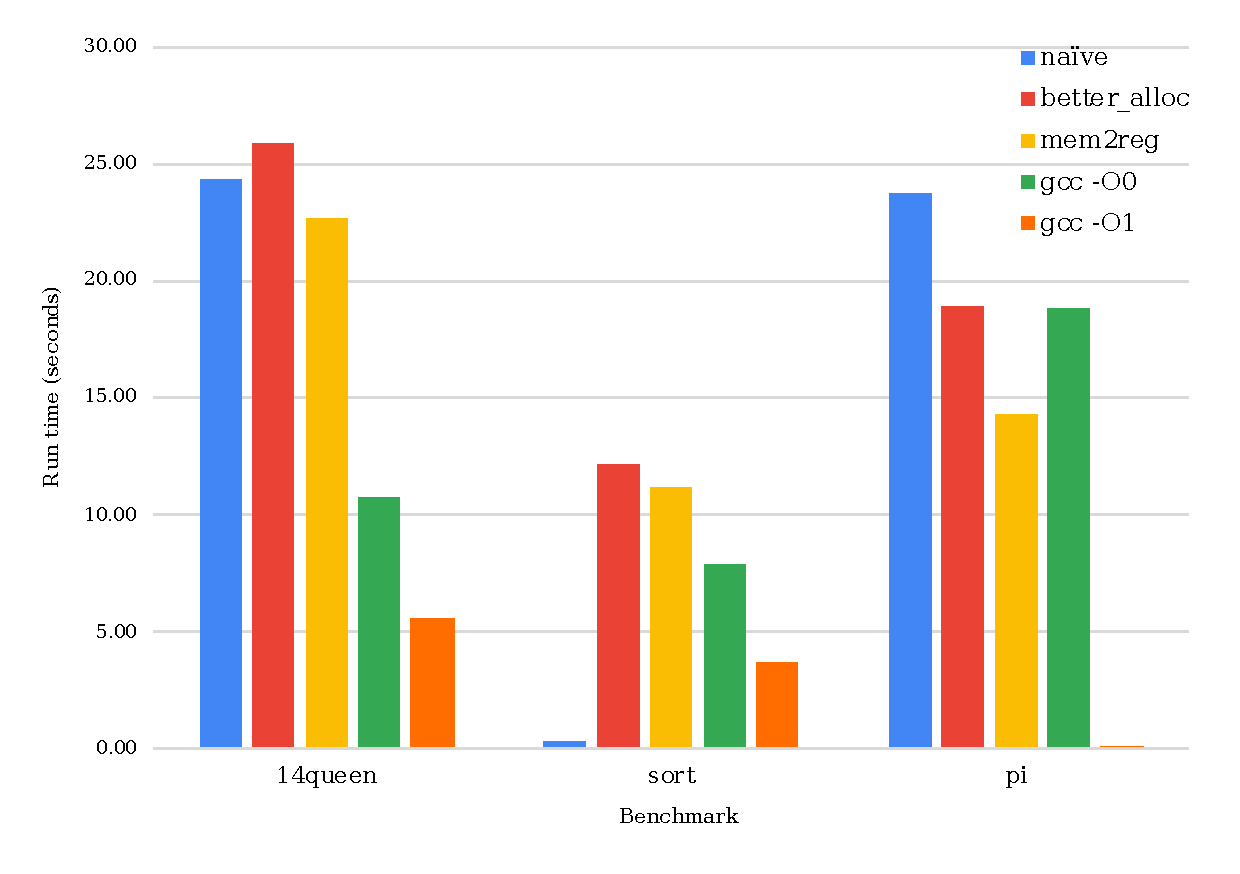
\includegraphics[width=15cm]{graph1.pdf}
  \caption{コンパイラごとの実行時間の比較}
  \label{ccc_bench_run_graph}
\end{figure}

\clearpage
\paragraph{出力コード行数}

出力コード行数のベンチマーク結果を\cref{ccc_bench_loc}に示す。

\begin{table}[h!]
  \centering
  \begin{tabular}{l|rl|rl|rl|rl|rl}
    &\multicolumn{10}{c}{行数 (gcc -O0との比)} \\ \hline
    &\multicolumn{2}{c|}{naive}&\multicolumn{2}{c|}{better\_alloc}&\multicolumn{2}{c|}{mem2reg}&\multicolumn{2}{c|}{gcc -O0}&\multicolumn{2}{c}{gcc -O1} \\ \hline\hline
    14queen&673&(2.50)&656&(2.44)&630&(2.34)&269&(1.00)&250&(0.93) \\
    sort&747&(2.46)&709&(2.33)&655&(2.15)&304&(1.00)&253&(0.83) \\
    pi&234&(2.07)&217&(1.92)&199&(1.78)&113&(1.00)&42&(0.37) \\
  \end{tabular}
  \caption{ベンチマーク結果: 出力コード行数}
  \label{ccc_bench_loc}
\end{table}

\section{展望}

当然ながらcccはどのベンチマークにおいてもgccよりも速くコンパイルできている。
cccの方が高速なコードを出力しているケースにおいても、最適化を行っていない\texttt{gcc -O0}と比べて最適化を行ったcccの方が高速にコンパイルできている。
効率よくコンパイルするという目標はよく達成できていると思う。\footnote{自己満足の話であり、gccより効率が良いと言いたいわけではない。}

その一方で実行時間については、ほとんどのベンチマークでgcc -O0より遅いという結果になった。しかしmem2regがpiでgcc -O0より高速なコードを出力できている。
これは14queenとsortが配列に対する操作が基本となるベンチマークであるのに対し、piはスカラ変数に対する操作が中心であることに起因すると考えている。
配列操作はどうしてもメモリアクセスが必要となってしまうが、スカラ変数に対する操作はmem2regでレジスタ操作に置き換えることができる。そのためpiではmem2reg最適化の効果が強く出たのではないかと考えられる。

また、\cref{ccc_bench_loc}を見ると実行時間が遅い項目は出力コード行数も多くなっていることがわかる。
したがって、cccをより高性能なコンパイラにするために、今後は出力命令数を減らすためにIR命令セットの再検討を行いたい。
また、mem2reg以外のloop unwindingや末尾再帰などの最適化パスも実装し、最終的にgcc -O1に主要なベンチマークで勝利できるコンパイラを目指す。

\section{結論}

あ〜

\clearpage
\appendix

\section{図表目次}
\listoffigures
\listofalgorithms
\listoftables

\bibliography{references}
\bibliographystyle{junsrt}

\end{document}
